\chapter{Approach}
In this chapter we will discuss in detail the approach we took to model the market and how it was implemented in order to plot the simulations. First we will start by mentioning that the language used for the simulations was python since it offers flexibility and prototyping can be done in a rapid manner. 

This chapter will be divided into two main parts, one detailing the code and its implementation and the second one we will present a flow chart in order to visualise it. Because of its complexity we will present a simplified version of the code with their most important components. The whole code and documentation can be found in the repository.


\section{Implementation}

The code can be divided into four parts: the imported libraries, the global variables needed for the model, the simulation algorithm and lastly the plotting of the simulation. In the next section we will describe each one of them and highlight its importance in the code.

It is worth noting that during the implementation due to time constraints, code length and very high simulation times we coded the model with the categories C1 and C2 and left C3 out. In the source code it can be found where the category C3 is yet to be implemented and can be easily added. In the chapter conclusion and improvements we will discuss this topic in more detail.

\subsection{Libraries}

For the calculation of the computation of the Poisson processes and exponential distributions we will use the library random from numpy. We can calculate get a random point from an exponential distribution by using the method exponential(). So if we were to type random.exponential(1/$\lambda$) we would get a random point from the exponential distribution of 1/$\lambda$. The same applies for a Poisson process. We can also get a random point from a Poisson process by calling the method Poisson($\lambda$,n) from random. Where n is the size and the first value is just a $\lambda$. This two methods will be used in order to calculate the arrivals of the agents as well as their maximum waiting times. 

The next library we used is Probability from PyProbs. This library will return a boolean with certain probability. The application for this is in the probability computation of the agents decision to take or leave a matched apartment. For this we can simply call Probability.Prob(x) where x represents a number between 0 and 1. As an example for x = 30, the method will return true 30\% of the time and false the other 70\%.

Lastly the library pyplot from matplotlib will help us with the plotting of the data.We will use mainly 2 methods from here. Pyplot.plot() which plots a set of arrays and Pyplot.table() which shows a set of arrays as a table. Other methods user are leyend(), lable(), title(), figure() among others. This last methods will set the legends, titles and make the plots easy to understand.

\begin{lstlisting}[language=Python]
import matplotlib.pyplot as plt
from numpy import random
from PyProbs import Probability as pr
\end{lstlisting}

\subsection{Global Variables}

In this section we will introduce the main global variables needed in order for the simulation to work properly. For the probabilities we will define a set of variables with the same syntax as in the one mentioned in the chapter one of this paper. The variables we can directly influence are pTC1, pTC2 and pTC3. this variables will contain whole numbers denoting the probability in \% of an agent choosing to take the accommodation. Moreover we will define the variables lambda\_c1, lambda\_C2, lamnda\_C3 and lambda\_Agents which will be our lambdas for the Poisson processes as well as a mWaiting (maximum waiting time) for an exponential distribution to calculate the maximum time an agent will wait to find accommodation before leaving the market.



An agent is stored in a python dictionary with an ID number in order to find it later. Then the agent in its self is again a dictionary with seven variables. This variables are "arrival" to store the arrival of the agent to the market, two booleans, "found" and "left" that states if the agent already found accommodation and if he has left the market. Then a dictionary to store the matched apartments to check later. Lastly he has a maximum waiting time and a variable to count the time he has already waited.
\begin{lstlisting}[language=Python]
agent = {
                    "arrival"   : t,
                    "found"     : False,
                    "category"  : "empty",
                    "waitingT"  : 0,
                    "maxWait"   : random.exponential(scale=mWaiting),
                    "offers"    : {},
                    "left"      : False
                }
                
agents{ID : agent}
\end{lstlisting}

The landlord-agents are stored the same way as the agents in a dictionary. First the ID number followed by the agent. The agent again is a dictionary this time with four variables. A waiting time and an arrival time as well as two booleans that also states if the agent has found a tenant or left the market.

\begin{lstlisting}[language=Python]
landlord = {
                    "arrival"   : t,
                    "found"     : False,
                    "waitingT"  : 0,
                    "left"      : False
                }
landlords{ID : landlord}
\end{lstlisting}

Lastly we will define a length of the experiment as in how many iterations will be done before the simulations stops. We will also define a set of arrays to store our KPIs some of these are, ratios and waiting times that in the end will be plotted.

\subsection{Simulation}

After the main variables are defined we can then start programming the algorithm for the model to work. First we will calculate the points in time where agents will arrive to the market during the whole experiment length (in iterations) and store them in a array. By calculating the exponential distribution of 1/$\lambda$ of the Poisson process we know how much time the agent will have to wait since the last agent arrival to the market. Then when we run through the iterations and we will know how many agents will arrive at that time. This initialization is analogous for the arrivals of apartments too.
\begin{lstlisting}[language=Python]
arrivalTimesTenants = []
counter = 0
mT = 1/lambda_Agents
while counter < expLength:
    x = random.exponential(scale=mT)
    counter += x
    arrivalTimesTenants.append(int(counter))
\end{lstlisting}

After having set the arrival times of the agents we will proceed to start the simulation. We will assume that a converging point is already known and will be denoted as expLength. The code is divided into two major iterations. The first one iterates over the variable interval (that being a lambda or a probability) that will be plotted as x axis. The second one iterates over time with the given variable and sets the simulation with this value. Next we can find a simplified code example for plotting over $\lambda$A with interval (0 to 10 in this example) that computes the arrivals of the agent to the market. On the second iteration we will set the experiment length to 1000 iterations.

The first loop uses the methods to set the arrival times for the agents as shown in the previously exposed code extract. Then the Dictionaries agents and landlords are initialised. The second loop has a set of simplified functions that executes the  simulation. 

The following functions are needed for the simulation:

\begin{itemize}
        \item \textbf{addAgentsToMarket()}: gets a list of agents with the times and amount of arrivals per iteration. Adds the new agents to the dictionary agents. Returns a list of the added agents in the current iteration.
        \item \textbf{addNewAgentsToFCFS()}: has as input the list of new agents added to the market, adds them to the matching system of C1 (FCFS).
        \item \textbf{matchAgentsToC2 ()}: recieves the dictionary of landlords and agents, match every agent to all available appartments in C2 (with probability \textbf{pMC2}.
        \item \textbf{matchAgentsToC1()}: recieves the list of landlords and FCFS queue. Gives the first the first agent in the queue the chance of a house \textbf{pMC1} and then has to choose either to take it or leave it with probability \textbf{pTC1}. If the agent takes it then he stops searching for accommodation, else goes back to the queue in last position. 
        \item \textbf{perishingAgents()}: from the dictionary of agents gets the agents that have one more iteration before perishing. Before the time runs out and have to leave the market.
        \item \textbf{lastOportunityMatch()}: iterates through the list of agents that are about to perish and searches in their list of matched apartments in C2 (dictionary "offers" in agents attributes) and if one option is still available the agent will take it with probability \textbf{pTC2} and stops searching for accommodation else the agent leaves the market and perishes.
        \item \textbf{incrementWaitingTime()}: goes trough the list of agents and increments the waiting time to those agents that are still searching and haven't left the market. Returns a list of the agents that perished.
        \item \textbf{leaveMarket()}: receives a list of agents that perished and the dictionary of agents. Sets the attribute "left" of the agent to true.
        \item \textbf{fillRatios()}: Computes the KPIs described in the introduction and waiting times and stores them. Plot() receives this data and plots it.
\end{itemize}

\begin{lstlisting}[language=Python]
expLength  = 1000
dataPoints = []
i = 0
while i < Lambda_A
    arrivingTimesAgents[] = setAgentsArrivalsLambda(i)
    arrivingTimesC1[]     = setC1Arrivals()
    arivingTimesC2[]      = setC2Arrivals()
    agents    = {}
    landlords = {}
    j = 0
    While j < expLength 
        newAgents = addAgentsToMarket(arrivingTimesAgents)
        addNewAgentsToFCFS(newAgents)
        matchAgentsToC2(landlords, agents)
        matchAgentsToC1(landlords, FCFS)
        perishingAgents = findAgentsPerishing(agents)
        lastOportunityMatch(perishingAgents)
        perishedAgents = incrementWaitingTime(agents)
        leaveMarket(perishedAgents, agents)
        j += 1
    KPI = fillRatios(landlords, agents)
    dataPoints[i] = KPI
    i += 1
plot(x, y, dataPoints)
\end{lstlisting}



\subsection{Plotting}

After the simulation is done it will start with the methods for the plotting of the result. These takes an x and y axis as well as an array of the points. A title and the name of the object figure and a legend. Lastly with the method plot and show we are redirected to a user interface where we can review the data. Here we will be able to adjust the plot to the desired intervals and zoom in or out on points of interest. Then we can choose a destination and save the data as PNG or JPG.

\begin{lstlisting}[language=Python]
plt.figure()
plt.title()
plt.xlabel()
plt.ylabel()
plt.plot()
plt.legend()
plt.show()
\end{lstlisting}

In order to fit this papers purpose the code has been highly simplified and separated into a set of general purpose functions. To see the full documentation and code implementation please refer to the git.

Now that we have explained in detail the working of the python code we can make a flowchart in order to represent it in its entirety. In the next section we can find the mentioned flowchart that visualises the previously described code. 

\newpage
\section{Flow Chart}
\begin{figure}[ht]
\centering 
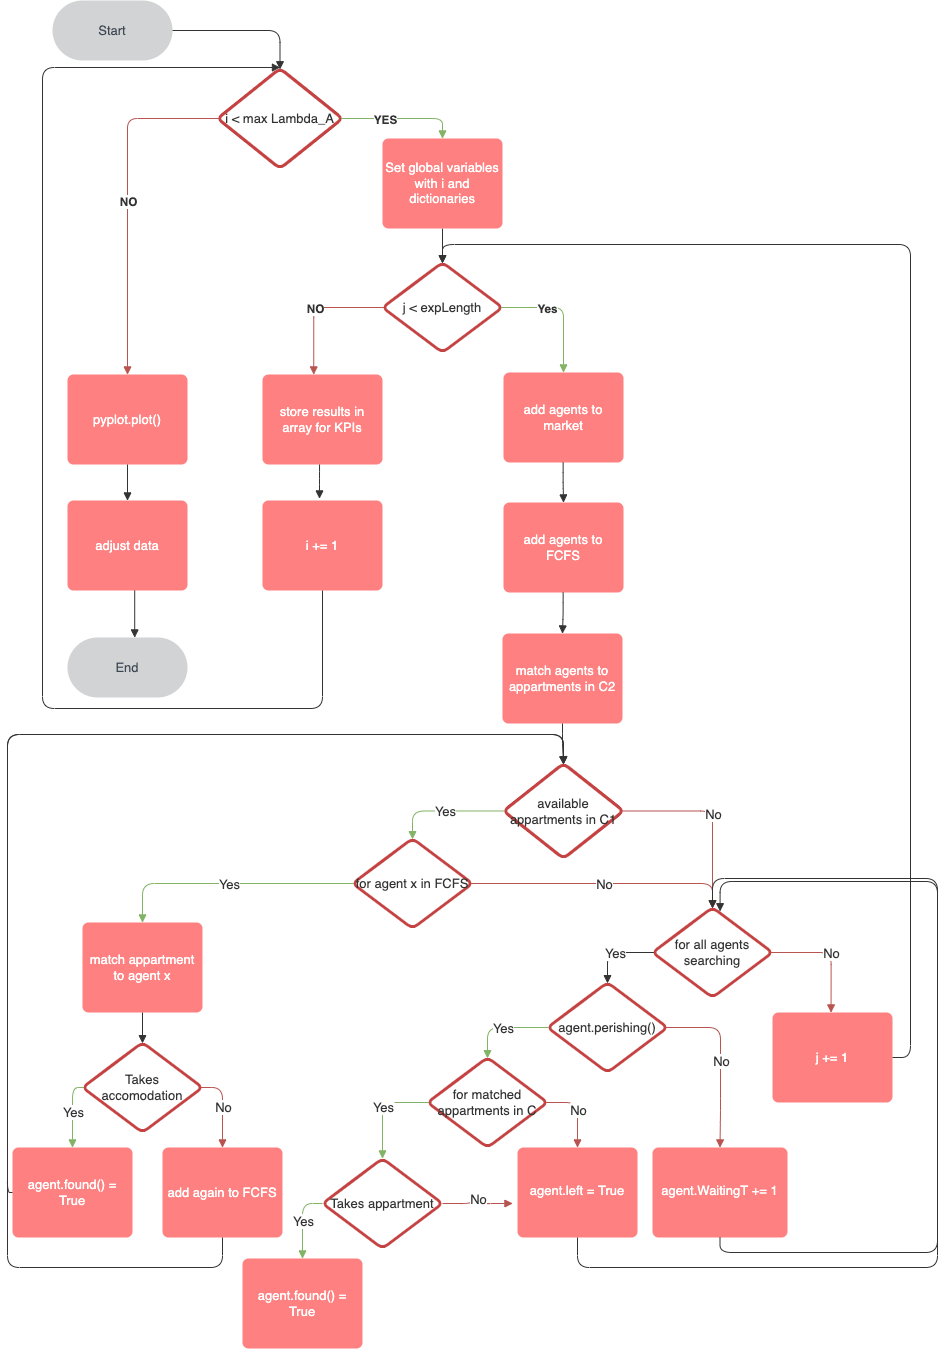
\includegraphics[width=0.71\linewidth]{figures/Flowchart.png}
\caption{The picture above encloses the code exposed in this chapter as a flowchart.}
\end{figure}
